\chapter{identPy: a Software for Parameter Estimation}

\label{ch: software}

In order to estimate the parameters of mathematical models, such as the one presented on chapter \ref{ch: Mod}, a python library called \textit{identPy} was developed by the author. \textit{identPy} implements a customizable framework for parameter estimation with built-in mathematical models and estimation methods. 

With this tool, comparison between performance of methods and precision of models can be easily done. Also, users are allowed to customize or create new features to match their needs without having to rewrite the entire framework, reducing time spent on coding. A Graphical User Interface (GUI) was developed as well, providing a simple environment where users can apply the estimation tool without any contact with the code.

The entire library and GUI were written in Python 3, a powerful, simple and fast high-level programming language that has gained large space in various sectors of industry and academy. Its rise is due mainly to the enormous number of libraries and forums developed and maintained by the users. Some examples of libraries used in this project are \textit{numpy} (for scientific computing), \textit{matplotlib} (graph plotting) and \textit{PyQt} (GUI toolkit). Also, python is open-source, not requiring a paid software to code and most of its applications are free.

The following sections describe how the library is organized and illustrate the estimation process using \textit{identPy} GUI.

\section{\textit{identPy} Library}

TODO.

\section{\textit{identPy} GUI}

The starting window will display some information about the software and the parameter estimation process, as shown in Figure \ref{fig: init_pg}.

\begin{figure}[h]
	\caption{Representation of software starting window}
	\begin{center}
		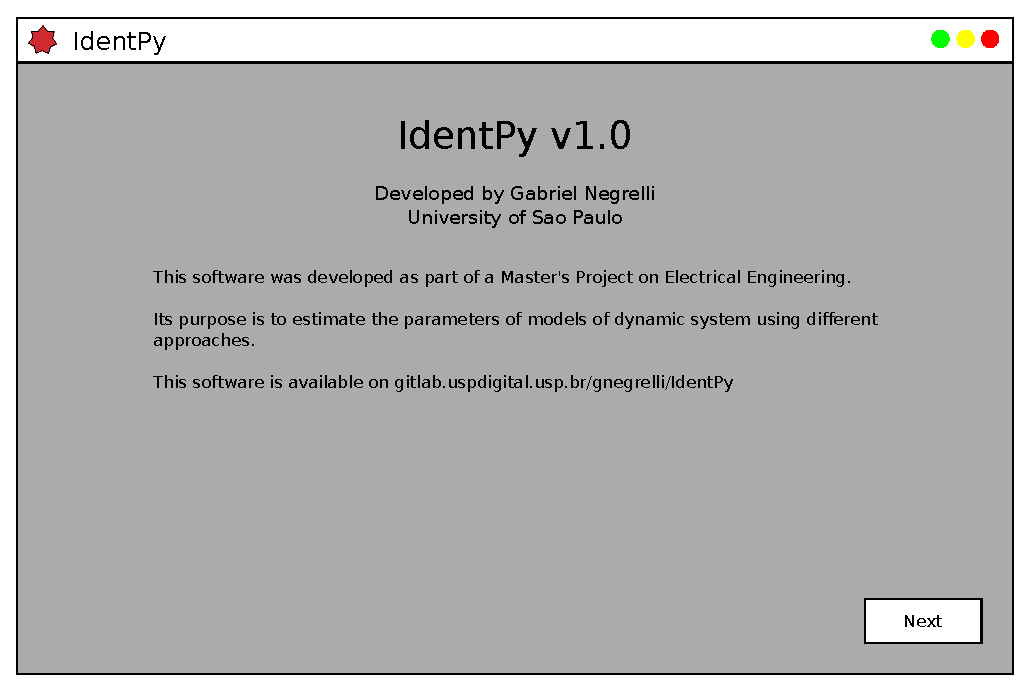
\includegraphics[scale=.5]{Images/Software_init_pg.eps}
	\end{center}
	\label{fig: init_pg}
\end{figure}

Next, the user will choose, from a list, which mathematical model will be employed, as depicted in Figure \ref{fig: pg1}. 

\begin{figure}[h]
	\caption{Representation of model selection window}
	\begin{center}
		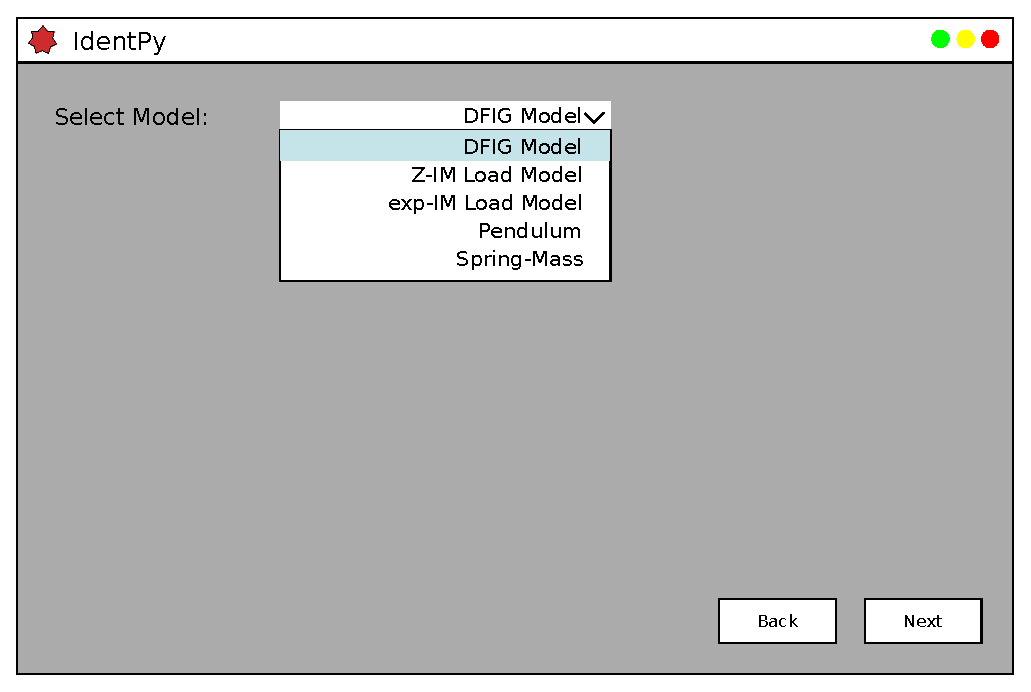
\includegraphics[scale=.5]{Images/Software_pg1.eps}
	\end{center}
	\label{fig: pg1}
\end{figure}

After that, a list of identification methods will be presented and the user will be able to select two methods, as displayed in Figure \ref{fig: pg2}.

\begin{figure}[h]
	\caption{Representation of method selection window}
	\begin{center}
		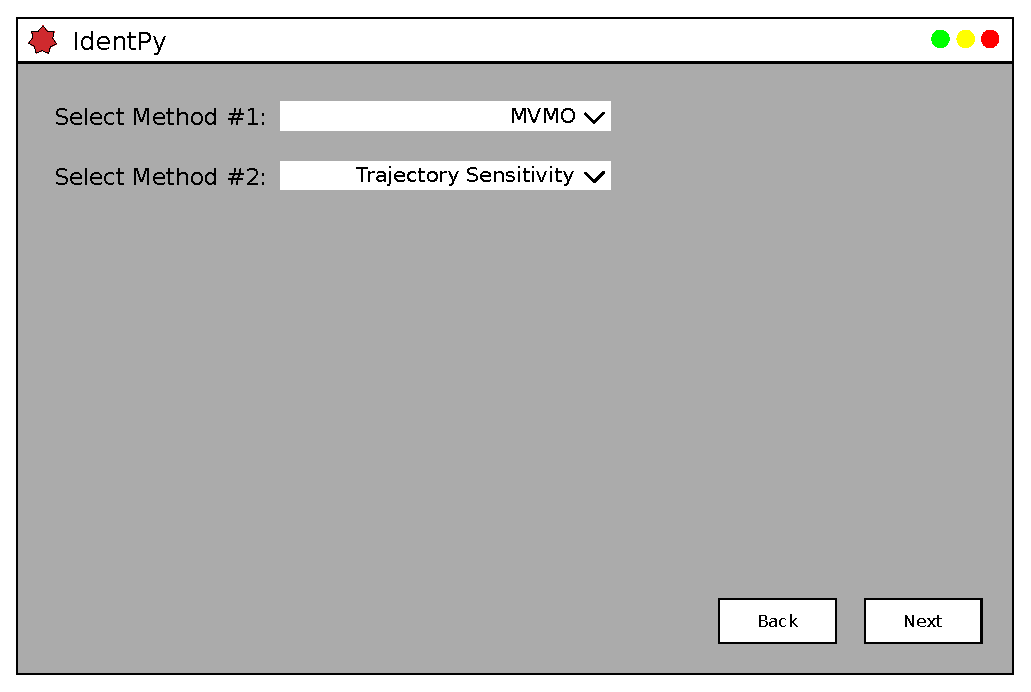
\includegraphics[scale=.5]{Images/Software_pg2.eps}
	\end{center}
	\label{fig: pg2}
\end{figure}


The settings of the chosen methods will done on the following windows and, finally, the user will enter the file containing the real system data and point out which data will be used as inputs and outputs. These steps are shown in Figures \ref{fig: pg3} and \ref{fig: pg4}, respectively.

\begin{figure}[h]
	\caption{Representation of method setting window}
	\begin{center}
		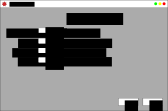
\includegraphics[scale=.5]{Images/Software_pg3.eps}
	\end{center}
	\label{fig: pg3}
\end{figure}

\begin{figure}[h]
	\caption{Representation of file selection window}
	\begin{center}
		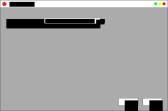
\includegraphics[scale=.5]{Images/Software_pg4.eps}
	\end{center}
	\label{fig: pg4}
\end{figure}

With all set, the estimation process will start and, at its end, a report will display the estimated parameters and the comparison between real system and model behaviours. The final view is represented in Figure \ref{fig: final_pg}

\begin{figure}[h]
	\caption{Representation of report window}
	\begin{center}
		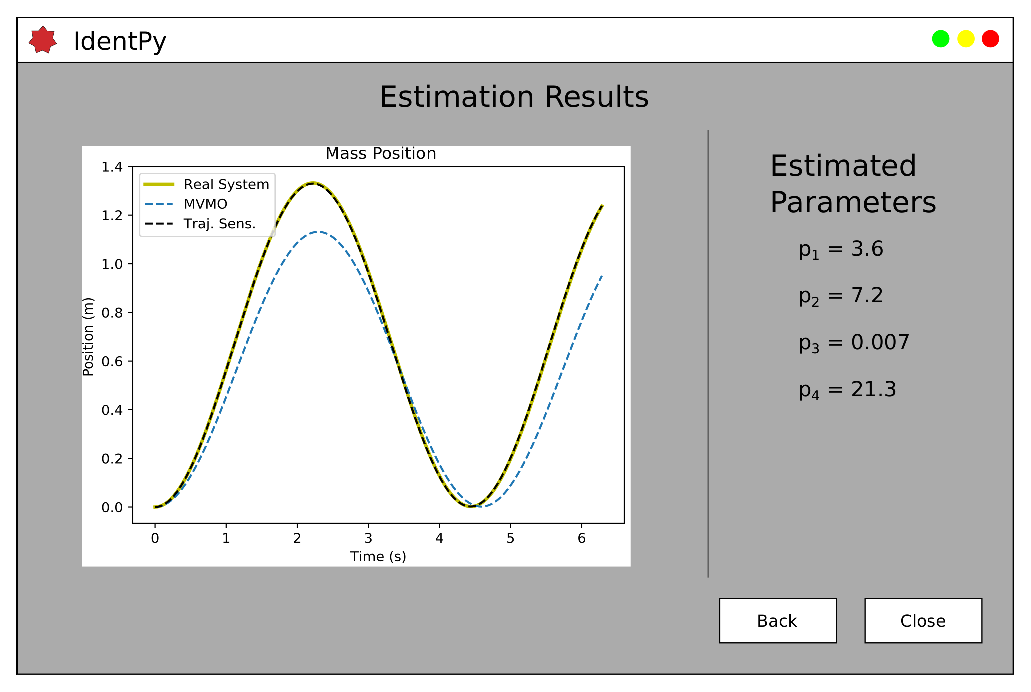
\includegraphics[scale=.5]{Images/Software_final_pg.eps}
	\end{center}
	\label{fig: final_pg}
\end{figure}

The order presented is not definitive and may change throughout the project if needed. However, all the steps discussed are core to the estimation process and cannot be discarded. Also, some other steps may be included in order to improve the software performance.